\documentclass[12pt]{report}
\usepackage{amsmath}
\usepackage{amssymb}
\usepackage{listings}
\usepackage{textcomp}
\PassOptionsToPackage{hyphens}{url}
\usepackage[breaklinks=true, naturalnames=true]{hyperref}
\usepackage{graphicx}
\usepackage{natbib}
\usepackage{color}
\usepackage{epigraph}
\usepackage[nottoc]{tocbibind}
\usepackage{amsthm}
\usepackage[ruled,vlined]{algorithm2e}
\usepackage{float}
\usepackage{tikz}
\usetikzlibrary{shapes.multipart, positioning, fit}

\hypersetup{colorlinks,citecolor=magenta,linkcolor=blue,urlcolor=blue}

\interfootnotelinepenalty=10000

%% \setlength\epitextskip{2ex}
\setlength\epigraphwidth{.8\textwidth}
\setlength\epigraphrule{0pt}

\newcommand{\namesigdate}[2][5cm]{%
  \begin{tabular}{@{}p{#1}@{}}
    #2 \\[2\normalbaselineskip] \hrule \\[0pt]
    {\small \textit{Signature}} \\[2\normalbaselineskip] \hrule \\[0pt]
    {\small \textit{Date}}
  \end{tabular}
}

\lstset{
  frameround=fttt,
  numbers=left,
  breaklines=true,
  keywordstyle=\ttfamily\color{blue}\bfseries, 
  basicstyle=\ttfamily\color{black}\bfseries,
  numberstyle=\ttfamily\color{black}\bfseries
}

\theoremstyle{definition}
\newtheorem{definition}{Definition}[section]

\lstloadlanguages{Haskell}
\lstnewenvironment{code}
                  {\lstset{}%
                    \csname lst@SetFirstLabel\endcsname}
                  {\csname lst@SaveFirstLabel\endcsname}
                  \lstset{
                    basicstyle=\small\ttfamily,
                    flexiblecolumns=false,
                    basewidth={0.5em,0.45em},
                    literate={+}{{$+$}}1 {/}{{$/$}}1 {*}{{$*$}}1 {=}{{$=$}}1
                    {>}{{$>$}}1 {<}{{$<$}}1
                    {\\\\}{{\char`\\\char`\\}}1
                    {->}{{$\rightarrow$}}2 {>=}{{$\geq$}}2 {<-}{{$\leftarrow$}}2
                    {<=}{{$\leq$}}2 {=>}{{$\Rightarrow$}}2 
                    {\ .}{{$\circ$}}2 {\ .\ }{{$\circ$}}2
                    {>>}{{>>}}2 {>>=}{{>>=}}2
                    {|}{{$\mid$}}1               
                  }
                  
                  \renewcommand{\lstlistingname}{Code snippet}
    
\begin{document}
    
    
\begin{titlepage}
\begin{center}        
\LARGE
\textbf{Elephant Tracks II: Practical, Extensible Memory Tracing}
        
\vspace{0.5in}
\large
by
\vspace{0.5in}

\Large
Xuanrui (Ray) Qi

\vspace{0.25in}

\normalsize
B.S.C.S., Tufts University, 2018

\vspace{1in}

\normalsize
A senior honors thesis\\~\\
submitted to\\~\\
the Department of Computer Science\\
School of Engineering\\
Tufts University\\
Medford, Massachusetts\\~\\
May 3, 2018

\vspace{0.75in}

\normalsize
\textbf{Thesis Committee:}\\
Professor Samuel Z. Guyer, Chair\\
Professor Kathleen Fisher
        
\end{center}
\end{titlepage}

\newpage
\vspace*{\fill}
\noindent
ELEPHANT TRACKS II: PRACTICAL, EXTENSIBLE MEMORY TRACING\\~\\\\~\\
Copyright by Xuanrui (Ray) Qi, 2018\\~\\\\~\\
This thesis is licensed under the Creative Commons Attribution 4.0 International (CC BY 4.0) License.\\
For a copy of the license, please visit: ~\url{https://creativecommons.org/licenses/by/4.0/legalcode}.\\~\\\\~\\
This thesis is typeset using \LaTeX.
\vspace*{\fill}
\thispagestyle{empty}

\newpage
\section*{\centering Abstract}
This thesis presents a new tool for memory tracing, Elephant Tracks II. Elephant Tracks II (or ET2) is a portable, modular and
extensible memory tracing tool designed for practical memory tracing of garbage-collected programs, producing precise traces of the
program's heap operations, including allocation, pointer mutation, procedure entry \& exit, and object deaths, using the Merlin algorithm
\citep{Merlin} to compute death times. Unlike all previous tools, however, ET2 is capable to support multiple programming languages by
decoupling the tracing phase and the death time computation phase. We describe the high-level design and low-level implementation
strategies employed to support this extensibility and portability. In this thesis, we also present new algorithms and implementation
techniques developed as part of the Elephant Tracks II project, as well as an overview of the applications of memory tracing.

\thispagestyle{empty}

\newpage
\section*{\centering Acknowledgements}
First of all, I must thank my advisor and thesis supervisor, Professor Sam Guyer, for his support. On a winter day,
I walked into his office and asked if he had research projects; Sam was kind enough to offer me many
potential projects. After a few steers, now here we are.  I shall also thank Professor Kathleen Fisher,
who, as a member of my thesis committee, the CS department chair, my programming languages (COMP 105) professor,
and a mentor of mine, was always helpful and caring. I need to also thank Dr. Michael Shah, now
a lecturer at Northeastern University, who was once a marvelous teaching assistant who connected me with Sam;
without him, I might not have been here at all. Finally, I must also thank Karl Cronburg, Raoul Veroy, Moses Huang,
Diogenes Nunez, Jared Chandler, Brian LaChance, Matt Ahrens, and Jeanne-Marie Musca for their assistance and support.
Two fellow undergraduates, Jeremy Colebrook-Soucie and Matt Jones worked with me on a different but closely related
project, ``JumboViz'' (as I call it), and their work on that project also proved to be helpful for the ET2 research
I am doing.

I must also thank my external collaborators who helped me on this project. I owe a lot to Luis Mastrangelo, who, as the author of the
JNIF library, provided us generous help and helped us debug our code. Kathryn McKinley and the DaCapo project group at Google also helped
with the Java version of ET2. Ben Gamari helped with the Haskell version of ET2. Without them, it would be difficult for me
to carry out my research.

Of course, there are many others whom I must thank. Without Professor Mark Sheldon, I wouldn't
have gone this far in computer science, and especially not in programming languages. Other faculty
in the computer science department, such as Professor Norman Ramsey, Professor Noah Mendelsohn, Professor Ming Chow, and the
much beloved Professor Ben Hescott, have also supported me as an undergraduate at Tufts. Finally, I shall not neglect to
thank the staff of the computer science department, who have always been helpful. Many, many more people supported me
during the course of this project and during my entire undergraduate career, but due to space limitations I could not possibly
list all of them here, so I'd like to apologize sincerely to all of those whom I have neglected to thank above. 


\setcounter{tocdepth}{0}
{\hypersetup{linkcolor=black}
 \tableofcontents
}
\thispagestyle{empty}

\setcounter{page}{0}
\chapter{Introduction}
\epigraph{\itshape A LISP programmer knows the value of everything, but the cost of nothing.}
         {---Alan J. Perlis, ``Epigrams on Programming'' (1982)}

\nocite{Epigrams}
         
\section{The cost of cost}
Most if not all reasonably experienced programmers would probably have programmed in a programming language with
manual memory management, especially C and C++. Few of those programmers would like to be reminded about the horrors
of debugging and facing memory bugs --- especially those caused by dangling pointers and memory leaks. Often times,
C programmers fail to know the \emph{value} of things --- this causes many memory bugs like dangling pointers and
out-of-bounds access. One must allocate the correct amount of memory and deallocate that memory at the right time ---
if the programmer ever makes a mistake, the value goes away.

In Perlis' time, programming in manually managed languages such as C, Fortran and Pascal was still the norm. However, had Perlis
lived through the 1990s, he would have rephrased his epigram as ``most programmers know the cost of nothing''.
For a Lisp --- and Java, Ruby or Haskell --- programmer, knowing the value of things are much easier. The days where an
off-by-one error may result in the program hitting garbage memory and giving out unexpected results were long gone, and, except
in the few cases where C programming is still necessary, the majority of programmers are using automatically (or at least
semi-automatically, as in the case of C++) managed languages.

Knowing the value of things is now much easier: structured, high-level programming languages have greatly decreased the chances
that inadvertent programmer errors result in fatal program errors. However, there is a trade-off in any engineering problem, and the
case of programming language choice is no exception. With these programming languages, the \emph{cost} of things become
largely unpredictable.

A Java or Haskell programmer might use heap-allocated, linked data structures, but they would never explicit allocate or deallocate
any memory. When the programmer creates a new class instance or a new algebraic data type instance, the runtime system manages the
allocation for the programmer. When the object becomes unreachable, the garbage collector finds it and calls \lstinline{free} for
the programmer. High level imperative programming languages like Java and functional programming languages Haskell thus allow programmers
to concentrate on value of the things, but as a ``side effect'', these programmers cease to understand the cost of things, which is
abstracted away from them. 

\section{Why cost matters}
Memory cost becomes intractable for those programmers. When programmers no longer understand the memory cost of program operations,
memory bugs and other issues might occur. For example, when a Java programmer creates a \lstinline{static} class member holding large
chunks of memory, or when they create streams and handles without closing them, memory leaks may occur. Here are two examples of
two Java programs that create memory leaks:

\begin{lstlisting}[
    caption={Java memory leak examples},
    label={lst:1}, basicstyle=\small,
    frame=single,
    numbers=none,
    language=java]
  // memory leak by static reference
  static List<Object> p = new ArrayList<>(33554432);
  
  // memory leak by held resource
  public void foo() {
      try {
          Connection conn = getConnection();
          // do something with the connection
          conn.close();
      } catch (Exception e) {
          // if an exception is thrown, close() is never called
          System.err.println("Error: " + e);
      }
  }
\end{lstlisting}

In C or C++, memory leaks are, despite being much more numerous, relatively easier to deal with as they are easier to spot and could
be found using tools like \emph{valgrind}. In most cases, a programmer only needs to find a \lstinline{malloc} call that is not paired
with a \lstinline{free} call. However, in Java, memory leaks are infrequent, but they are hidden and might have serious consequences if
not discovered. A Java programmer might know when and where their object is allocated, but they almost never know when their object dies.
Moreover, the garbage collection overhead adds an indeterminable cost to program execution; although there are effective methods to decrease
this cost with some programmer input \citep{NG2C, PrioritizedGC}, the ``why'' is often not adequately understood.

For a Scala or Haskell programmer, the situation might be even worse as the basic program operations do not directly map into
memory allocations and deallocations. In this case, it is extremely hard for programmers to understand, and sometimes impossible,
for programmers to analyze the cost of their program operations. Although functional programming languages are not designed to be
memory efficient, sometimes the cost of programs is simply too large to be ignored. For example, due to lazy evaluation and
the use of function closures, a simple red-black tree benchmark in Haskell allocates more than 3 gigabytes of memory on the heap
(see Appendix A for the program). In comparison, both the Standard ML and OCaml versions of this benchmark, compiled using their
respective optimizing native-code compilers (MLton and \lstinline{ocamlopt}), allocate only about 1.6 gigabytes of memory, ostensibly due to
both SML and OCaml using eager evaluation. Most of the extra memory Haskell allocates is deallocated immediately, but at this scale,
the space cost of functional programs does deserve more comprehension.  

The goal of this thesis, therefore, is to help Lisp --- and Java, Scala, Haskell, etc. --- programmers overcome Perlis' epigram
by providing them with tools that can help them understand the cost of their programs precisely. More specifically, this thesis looks into the
dynamic analysis of the space cost of programs; that is, to help programmers understand the life and death of their heap objects
at runtime.

\section{Why memory tracing?}
To better understand memory usage patterns in programs and identify
potential memory bottlenecks, we could use dynamic analysis to generate memory traces, or records of lives and
deaths of objects dynamically allocated on the heap. With those records, one could fully understand the memory usage
patterns of automatically memory managed programs.

Memory and garbage collection tracing is of paramount importance to the analysis of memory performance in garbage-collected
languages. Experimental studies of memory behavior and garbage collector performance \citep{ScalaJava, Garbology} rely on
precise analysis made possible by GC tracers. Moreover, memory tracing can be useful for debugging memory bugs and potential leaks
\citep{MemInsight}. Finally, memory tracing can be used to analyze the finer parts of GC performance issues, such as average
latency, i.e., time lapsed between the death of an object and its eventual deallocation.


\section{Challenges with preexisting tools}
Despite the importance of memory tracing in the analysis of garbage collection and memory usage in managed languages, there have
been few tools available to perform this task. One preexisting tool, GCTrace, is available as a component of the Jikes RVM \citep{JikesRVM}. However,
the Jikes RVM has been of research interest only, and has been mostly superseded by HotSpot JVM even in that field. Moreover, GCTrace
is built into the Jikes RVM and updates to the JVM itself has rendered it unusable in newer versions of Jikes RVM. Thus, GCTrace has
mostly been fell into disuse. Another tool, Elephant Tracks \citep{ElephantTracks}, comes from our previous work, and was designed with
the goal to be portable between different JVMs in mind; in practice, Elephant Tracks has proved to be a relatively trustworthy tool.

However, Elephant Tracks has three fatal flaws. First, Elephant Tracks is not well documented and standardized, so its trace output
format and code base could bit-rot quickly, and as a result often fails its design goal of portability. Second, Elephant Tracks can
only provide GC trace analysis for JVM languages as the death record generalization process is built in to the running Java program
as a JVM agent. Finally, Elephant Tracks, although precise, is extremely slow: in usual cases, Elephant Tracks slows down program execution
by 500-1000 times, making full analysis of larger programs impossible. Although Elephant Tracks has been a good tool for controlled
experiments on the Java GC, its usage is severely limited by performance and portability issues.


\section{Presenting a new tool}
Although efforts were made to refine Elephant Tracks, it proved difficult to substantially improve the tool. Specifically, Elephant Tracks
has many outdated dependencies with legacy APIs, and updating the dependencies requires substantial engineering effort. Moreover,
Elephant Tracks suffers from a significant architectural flaw: Merlin, the algorithm used to produce death timestamps,
is run during the trace collection phase. Naturally, this slows down program execution and limits attempts to enhance the extensibility
of Elephant Tracks. As a result, the only choice left is to mostly scrape Elephant Tracks and re-design Elephant Tracks from scratch
(while reusing some components of the old Elephant Tracks), hence our tool is named Elephant Tracks II. While running the same algorithms and
using the same trace-gathering mechanics as Elephant Tracks, Elephant Tracks II is architecturally very different from the original Elephant
Tracks.

In this thesis, we will present \emph{Elephant Tracks II} (ET2), a GC tracing tool and memory analysis framework that inherits many of
the goals of Elephant Tracks, but which is also substantially different from Elephant Tracks in many ways; ET2 could thus be considered
a successor to Elephant Tracks. 


\section{Goals of the Elephant Tracks II project}
The goals of the Elephant Tracks II project directly address the shortcomings of Elephant Tracks. The main design and implementation
goals of Elephant Tracks II are as following:

\begin{enumerate}
\item \textbf{standardization}: provide a standard interface to and output format for GC traces;
\item \textbf{efficiency}: be as fast as possible, with the goal being a 50-100 $\times$ slowdown (as compared to
  Elephant Tracks' 500-1000 $\times$ slowdown, this is really fast!);
\item \textbf{modularity}: be as modular as possible. Especially, we would like to decouple the Merlin algorithm from the
  JVM agent, moving it into the ``postmortem'' analysis phase, which does not affect program execution;
\item \textbf{inter-language operability}: a result of the improved modularity, the new Elephant Tracks II trace analyzer can
  now analyze GC traces from any language in principle.
\end{enumerate}


\section{Outline of the thesis}
The thesis will be divided into six chapters, excluding this introductory chapter. Chapter 2 will introduce the premliminaries and
past work, including the Merlin algorithm \citep{Merlin}, memory tracing techniques, and issues with earlier GC tracer designs,
especially issues concerning the design of the original Elephant Tracks. Chapter 3 will outline the architecture, trace format and
major design concerns in the design of Elephant Tracks 2. Chapter 4 will discuss the implementation of Elephant Tracks II, including
the major programming techniques and strategies used to deal with difficult situations. Chapter 5 will discuss the extensibility of
Elephant Tracks II and explore the possibility of using Elephant Tracks II to analyze the memory behavior of non-object oriented,
and especially functional languages. Chapter 6 will present experimental results using a series of benchmarks, including the DaCapo
benchmarks \citep{DaCapo}. Chapter 7 will provide a comparison to other work, outline future work, and conclude the thesis.


\chapter{Preliminaries and Previous Work}
\label{chap:prelim}
\section{The fundamental problem of garbage collection analysis}
Memory management is difficult, and the horrors of manual memory management need
not be reiterated. Reference counting is a simple alternative to manual memory
management, but suffers from two major drawbacks: (1) it incurs significant
runtime cost, as the reference count needs to be updated whenever a new alias is
created or destroyed for each pointer, and (2) it results in memory leaks whenever
cycles are formed in the reference graph. Graph-based garbage collection algorithms
fix both problems, and are easy to parallelize and optimize \citep{GCHandbook}.

Although garbage collection is a much more efficient algorithm than reference counting
for most purposes, it has a few serious drawbacks. Garbage collection algorithms,
no matter how refined, cause random pauses during program execution which are unpredictable
and nondeterministic. Moreover, garbage collctors cannot tell us when objects die; all we could
know is that garbage-collected objects die \emph{some time} between the last garbage
collection run and the current garbage collection run.

Thus, the properties of garbage collectors impede the analysis and evaluation of themselves, and
external tools are often required to analyze garbage collectors. For example, a good garbage collector
should minimize the time span $\Delta t$ between an object's death time $t_{d}$
and collection time $t_{c}$. A reasonable metric that a garbage collector designer (and implementer)
would like to minimize might be the average ``time to collection'', i.e.
\begin{equation} \label{eq:1}
  \overline{\Delta t} = \frac{1}{n_{obj}}\sum_{i=1}^{n_{obj}}(t_c^i - t_d^i)
\end{equation}

However, without extra analysis tools, one could not obtain even a reasonable guess for the
$t_{d}$ value of any object, and therefore could not compute $\overline{\Delta t}$ using \ref{eq:1}.
Obtaining death times for each object is (in principle) easy: for example, one could simply do
``mock'' reference count on each object (without actually deallocating dead objects) and
recording the object death times. Nevertheless, this method, albeit intuitive, suffers from
the same drawbacks that plague the effectiveness of reference counting: this will degrade runtime
performance (such that the validity of timestamps obtained become questionable), and this method
could not generate death records for objects that form part of a cycle in the reference graph.

For these reasons, neither Elephant Tracks II nor other GC tracing tools \citep{MemInsight, ElephantTracks}
use reference counting to generate death record. Instead, we use the Merlin algorithm \citep{Merlin}, which
will be discussed hereafter, to \emph{compute} precise object death records using information gathered
at runtime.

\section{The Merlin algorithm}
Instead of (painstakingly) building a reference counter into a runtime system and generate incomplete death
records with it, one could compute the \emph{idealized death time} of objects using the Merlin algorithm, which
is based on a simple insight. There are two ways that object ``die'', i.e. become disconnected from the reference
graph: when there are no more references to the object, or when all objects that hold references to the said object
have died \citep{Merlin, ElephantTracks}. Thus, we could compute the death time of each object recursively:
\newpage
\begin{lstlisting}[
    caption={Haskell-style pseudocode for the Merlin algorithm},
    label={lst:1}, basicstyle=\small,
    frame=single,
    numbers=none,
    language=haskell]
  deathTime :: Object -> Timestamp
  deathTime o = max (timeStamp o)
                    (maximum pointsToDeathTimes)
      where
      pointsToDeathTime = map deathTime (allPointsTo o)
\end{lstlisting}
where  \lstinline{allPointsTo o} generates a list of objects that point to \lstinline{o}, and\\
\lstinline{timeStamp o} fetches the ``timestamp'' for \lstinline{o}. For the purposes of the Merlin algorithm,
the \emph{timestamp} for an object is the last time at which the object is found to be accessible or ``alive''.

The na\"{i}ve recursive version of the Merlin algorithm is illustrative for purposes of understanding the
algorithm, but is inefficient for actual implementation. However, \cite{Merlin} also gives an efficient implementation, based
on depth-first search through the reference graph, that runs in $\Theta(n \log n)$ time and has good
experimental results. Additionally, although the Merlin algorithm is designed to run on each garbage collection,
it could also be run offline if garbage collections are recorded in the GC trace. In Elephant Tracks, the online
approach is used; however, in Elephant Tracks II, the offline approach will be used.

With the Merlin algorithm, the problem of generating death records is transformed into one of finding timestamps
for each object, but the Merlin algorithm itself leaves this as an open question. For Java-like languages, the
best marker of an object being alive is probably the object being ``used'', e.g. an instance method called on the
object, the object being assigned to a pointer, etc. However, the strategy used is up to the implementer, and
the effectiveness of Merlin is up to effective timestamp generation for each object.

\section{Elephant Tracks}
Elephant Tracks \citep{ElephantTracks} is the major motivation for the work in this thesis, and represents a major attempt
to use the Merlin algorithm for practical GC tracing. Elephant Tracks is implemented as a JVM Tool Interface (JVMTI) agent, or a shared library
containing callbacks for the JVM to call on a number of events, e.g. whenever a class is loaded.

To generate timestamps for each object, Elephant Tracks rewrites the bytecode of each class before it is loaded, and inserts
calls to methods that record significant events. For example, whenever Elephant Tracks find an object allocation in a method,
it inserts a call to a method that records the allocation event. Whenever Elephant Tracks finds a \texttt{getfield} instruction
in a method, it inserts a call to update the timestamp for the object subject to the instruction, as a \texttt{getfield} on an
object indicates the aliveness of the object.

When a class is about to be loaded, the JVM calls the callback function supplied to it,
while the function sends the bytecode to a bytecode manipulator process. The ``bytecode manipulator'' rewrites the class using
the ASM bytecode instrumentation library, and sends the instrumented bytecode back after it is done with instrumentation. Then, at
runtime, the new, instrumented bytecode will be executed, and records will be generated by the inserted ``interceptor'' methods. As
all production-level JVMs provide implementations of the JVMTI, Elephant Tracks is, in principle, compatible with all standards-conformant
JVM implementations.

While Elephant Tracks is mostly successful in generating precise and complete GC traces for Java programs, one may easily see that
the implementation of Elephant Tracks is extremely inefficient. First of all, inter-process communication between the agent and the
``bytecode manipulator'' is required on \emph{every single} class load, which adds extremely high overhead to the running Java program.
Moreover, the ``interceptor'' methods are all native methods, requiring the JVM to invoke the JNI on any ``interesting'' event. Finally,
this complex architecture has rendered the code base for Elephant Tracks no longer maintainable and extremely prone to bit-rot. In fact,
by February 2018, Elephant Tracks can only run on a very old version of IBM J9 JVM, using outdated versions of the ASM library, and can
slow down program execution by 800 to 1000 times. Initially, Elephant Tracks was proposed as a fast and portable alternative to its alternatives
such as GCTrace, but due to architectural and design flaws, Elephant Tracks no longer meets its initial design goals.

Our new tool, Elephant Tracks II, is a tool ``in the spirit of'' Elephant Tracks, but is free of many design flaws of Elephant Tracks, making
it easily extensible and maintainable.


\chapter{Architecture}
\label{chap:arch}
\section{The architecture of Elephant Tracks}
\cite{ElephantTracks} listed six design goals of Elephant Tracks: precise, complete, informative,
well-defined, portable, and fast. However, the latest release of Elephant Tracks \citep{ElephantTracksPage}
barely achieves three of those goals, namely well-defined, portable and fast.

According to \cite{ElephantTracksPage}, the current release of Elephant Tracks fails to run on most Java
implementations (supporting only IBM J9), does not support recent Java implementations, and can be
irritatingly slow. Most of the problems bugging Elephant Tracks could be attributed to its architecture.

The old Elephant Tracks --- like the new Java frontend to Elephant Tracks --- is written as a JVM Tool Interface
agent \citep{ElephantTracks}. The JVMTI, according to Oracle's specifications, is a interface which should be implemented
by all standards-conforming JVMs that allow developers and debuggers to dynamically inspect and control the state
and execution of Java programs \citep{JVMTI} running in a JVM, in a fashion similar to the GNU Debugger
(\lstinline{gdb})'s state inspection and execution control facilities. For example, \lstinline{jdb}, the
\lstinline{gdb}-style debugger included in both of Oracle's Java implementations (Oracle JDK and OpenJDK), is implemented
as a JVMTI agent.

The JVMTI does not specify how the JVM shall interact with JVMTI agents besides stating that they should ``run in the same
process with and communicate directly with the virtual machine executing the application being examined''. However, since
JVMTI agents are compiled to native shared objects on the host system, most if not all JVM implementations dynamically
link with the JVMTI agent at runtime and call into the JVMTI agent at specific events. For example, a (rather primitive)
profiler might want to set a callback on the entry and exit of each method to generate a call graph. At run time, every time
a method is entered or exited, the JVM calls into the provided callback function and executes it. The JVMTI, therefore, is an
ideal technique to implement a memory tracer. Thus, when we designed the Java frontend for ET2, we chose to continue to use
the JVMTI as a portable and efficient technique to gather traces.

Elephant Tracks uses dynamic \emph{bytecode rewriting} as its major implementation technique. A JVMTI callback is set such that
Elephant Tracks gets access to a class's metadata and bytecode right before a class is loaded. Then, Elephant Tracks inspects
the bytecode of each method in the class, searching for important events such as object allocation (i.e. a \lstinline{new} instruction)
or a pointer update (usually a \lstinline{putfield} instruction). When an important event is found, the bytecode rewriter inserts a
call to a static method in a ``proxy'' class. After Elephant Tracks rewrite the class, it is loaded and executed. During
execution, the ``proxy'' method generates appropriate traces for the event it witnesses.

For example, let us consider the following Java method, taken from a real benchmark used to profile ET2:
\begin{lstlisting}[
    caption={Elephant Tracks example: source code},
    label={lst:1}, basicstyle=\small,
    frame=single,
    numbers=none,
    language=java]
  public class BinarySearchTree<T extends Comparable<T> > {
      // other methods omitted
    
      public void insert(T insertVal) {
          if (val == null) {
              val = insertVal;
              return;
          }

          if (val.compareTo(insertVal) <= 0) {
              if (right == null) {
                  right = new BinarySearchTree<T>(insertVal);
              } else {
                  right.insert(insertVal);
              }
          } else if (left == null) {
              left = new BinarySearchTree<T>(insertVal);
          } else {
              left.insert(insertVal);
          }
      }
  }
\end{lstlisting}

An analysis at the source code level would allow us to spot the allocation sites and pointer updates and
``liveness witnesses'' (i.e. instructions that proves the liveness of an object) in the code:
\begin{lstlisting}[
    caption={Elephant Tracks example: annotated source code},
    label={lst:1}, basicstyle=\small,
    frame=single,
    numbers=none,
    language=java]

  public class BinarySearchTree<T extends Comparable<T> > {
      // other methods omitted
      
      public void insert(T insertVal) {
          // witness the liveness of the callee of ``insert''
        
          if (val == null) {
              // pointer update: val -> insertVal
              val = insertVal;
              return;
          }

          if (val.compareTo(insertVal) <= 0) {
            if (right == null) {
                  // allocation and pointer update
                  right = new BinarySearchTree<T>(insertVal);
              } else {
                  right.insert(insertVal);
              }
          } else if (left == null) {
              // allocation and pointer update
              left = new BinarySearchTree<T>(insertVal);
          } else {
              left.insert(insertVal);
          }
      }
  }
\end{lstlisting}


Next, the bytecode of the \lstinline{compile} method shall be examined. The \lstinline{BinarySearchTree} class
is compiled using \lstinline{javac} version 1.8.0\_161 and then disassembled using \lstinline{javap}. Comments which mark the places where
Elephant Tracks would inject method calls have been inserted.
\begin{lstlisting}[
    caption={Elephant Tracks example: annotated bytecode},
    label={lst:1}, basicstyle=\small,
    frame=single,
    numbers=none,
    language=jvmis]
  public void insert(T);
      Code:
         0: aload_0
         1: getfield      #2  // Field val:Ljava/lang/Comparable;
         4: ifnonnull     13
         7: aload_0
         8: aload_1
         // pointer update
         9: putfield      #2  // Field val:Ljava/lang/Comparable;
        // method exit
        12: return
        13: aload_0
        14: getfield      #2  // Field val:Ljava/lang/Comparable;
        17: aload_1
        // liveness witness (``val'') & method call
        18: invokeinterface #6,  2  // InterfaceMethod java/lang/Comparable.compareTo:(Ljava/lang/Object;)I
        23: ifgt          59
        26: aload_0
        27: getfield      #4  // Field right:LBinarySearchTree;
        30: ifnonnull     48
        33: aload_0
        // allocation
        34: new           #7  // class BinarySearchTree
        37: dup
        38: aload_1
        // method call
        39: invokespecial #8  // Method "<init>":(Ljava/lang/Comparable;)V
        42: putfield      #4  // Field right:LBinarySearchTree;
        45: goto          89
        48: aload_0
        49: getfield      #4  // Field right:LBinarySearchTree;
        52: aload_1
        // liveness witness (``right'') & method call
        53: invokevirtual #9  // Method insert:(Ljava/lang/Comparable;)V
        56: goto          89
        59: aload_0
        60: getfield      #3  // Field left:LBinarySearchTree;
        63: ifnonnull     81
        66: aload_0
        // allocation
        67: new           #7  // class BinarySearchTree
        70: dup
        71: aload_1
        // method call
        72: invokespecial #8  // Method "<init>":(Ljava/lang/Comparable;)V
        // pointer update
        75: putfield      #3  // Field left:LBinarySearchTree;
        78: goto          89
        81: aload_0
        82: getfield      #3  // Field left:LBinarySearchTree;
        85: aload_1
        // liveness witness ("left") & method call
        86: invokevirtual #9  // Method insert:(Ljava/lang/Comparable;)V
        // method exit
        89: return
\end{lstlisting}

As one might see, there are two deciding factors that constrain Elephant Tracks' efficiency: the efficiency
of bytecode rewriting, and the number (and efficiency) of inserted method calls. However, these two aspects
are exactly the places where Elephant Tracks perform badly.

In the Elephant Tracks workflow, a JVMTI callback fetches the bytecode of a newly loaded class, and then launches
a rewriting procedure (using the ASM library) in a new JVM process. The communication between the Elephant Tracks
host JVM and the newly lanched Java process is facilitated using standard UNIX interprocess communication utilities.
Then, the rewriter inserts a number of instrumentation method calls to the program. However, the instrumentation calls
are JNI invocations, and this results in the abstraction barrier between the JVM and the underlying system being broken
frequently, resulting in many important JVM facilities (such as just-in-time compilation) becoming unusable. The overheads of
interprocess communication and JNI invocations, when combined, results in poor performance for Elephant Tracks.

For details on the design of Elephant Tracks, however, we shall direct readers to \cite{ElephantTracks}. The main point here is
that the design of Elephant Tracks is driven by implementation and unmodular, and thus it contains a few important flaws which
need to be rectified. Thus, to optimize the workflow of Elephant Tracks, we propose a new design that decouples separate tasks
involved in memory tracing.

\section{Overview}
Elephant Tracks II contains two major components: the trace-collecting frontend, and the death-time computing backend. The two
components are completely decoupled from each other; as long as the frontend generates complete program traces in a 
Elephant Tracks II-compatible format, the backend will be able to compute accurate death records for the program trace, while the
accuracy of death records is completely up to the accuracy of the frontend. In other words, the backend is completely agnostic
about the frontend: the language of the program being traced and the method used to do tracing is irrelevant when it comes to
death time computation.

Elephant Tracks II is primarily designed for Java and other languages running on the Java virtual machine. For the sake of simplicity,
we will refer to \emph{both} the backend and the JVM frontend as ``Elephant Tracks II'' without qualification. However, Elephant Tracks II is not limited
to Java and the JVM: a frontend could be implemented for any programming language that use heap allocation, pointers, and garbage collection
\emph{at the implementation level}. Haskell, for example, does not have pointers or a memory model at the language level as all data is
immutable; however, heap allocation and pointers are used by the Glasgow Haskell Compiler to implement functional closures and lazy evaluation.
Thus, it is possible to use Elephant Tracks with the \emph{GHC implementation} of Haskell \footnote{However, if there was ever a
  implementation of Haskell which does not use pointers and heap-allocated memory in its memory model, such as an implementation
  directly on a SECD machine, we will not be able trace Haskell programs in that implementation. Fortunately, all practical Haskell
  compilers targeting the von Neumann architecture need to use heap allocation and pointers.}. Although we did not implement a Haskell
frontend for ET2 in the work leading to this thesis, we will describe a model for adapting ET2 to functional programming systems in
\hyperref[chap:extensible]{chapter 5}.

The algorithms and strategies used by the backend to compute death times will be described in the \hyperref[chap:algoimp]{next chapter}. In
the rest of this chapter, we will mainly discuss the high-level design of ET2.

\section{The ET2 frontend: trace collector}
Memory tracing is inherently slow, and the trace collector is where most of the problem is at. However, to safely optimize trace collection, we must
first decouple the trace collection phase from the computation phase. In the Elephant Tracks II architecture, the implementation of the
frontend, or trace collector, is not defined. Instead, the implementer may select whichever implementation technique that is appropriate. For Java,
we have continued to use bytecode rewriting as our main technique. However, for a native code compiler-based languages implementation like the GHC,
building trace-generation into the runtime might be a more appropriate technique.

To calculate object death times, five types of traces are required: procedure entry, procedure exit, object allocation, pointer updates, and \emph{witness}. Each trace must have a \emph{timestamp} which is necessary for running Merlin. A timestamp in the context of
ET2 is a logical timestamp that impose a total ordering on events; examples of good candidates for timestamps are the total number of 
method entries and exits, or the total number of allocated bytes. A physical timestamp, however, is not recommended as the trace
collector slows down program execution substantially. However, in the presence of concurrency, a total ordering on events might not be
appropriate. In that case, we could potentially use techniques such as Lamport clocks \citep{LamportClock} to induce a partial ordering
on events; however, this is still an open research problem\footnote{We will revisit this problem in the
\hyperref[chap:conclusion]{final chapter}.}.

The procedure entry trace has the following format:

\begin{verbatim}
M <procedure-id> <receiver-object-id> <thread-id> <timestamp>
\end{verbatim}

In case that the traced programming language is not object-oriented, or that the method is global (e.g. a static method in Java), the
\lstinline{receiver-object-id} should be 0. For a language without threading support, the thread ID could be 0.

The procedure exit trace has a similar format, only with the \lstinline{M} replaced by an \lstinline{E}. A procedure might be
exited due to either returning from the procedure or a thrown exception (as implemented by \lstinline{throw} in Java and
\lstinline{raise} in ML)
\footnote{Besides exceptions, other control operators, such as \lstinline{throw} in Standard ML, \lstinline{shift} in Racket and
  \lstinline{yield} in Lua, can also result in a procedure being exited without returning from the procedure. These should also be
  counted as method exits.}, and ET2 does not discern between these different types of exits.

The heap allocation trace has the following format:

\begin{verbatim}
<alloc-type> <object-id> <size> <type> <site> <length> <thread-id> <timestamp>
\end{verbatim}

There are two types of allocations: an allocation is either ``singular'' (as in allocating a Java object) or ``block'' (as in
allocating a Java array). An array allocation (denoted by \lstinline{A}) is deemed to have occured when a logically contiguous
section of memory is allocated for a sequential collection of objects (i.e. an array), and in all other cases an allocation is
singular (denoted by \lstinline{N}). The \lstinline{object-id} is an unique, numerical identifier which identifies a newly allocated
heap object, while \lstinline{site} is a globally unique, numerical identifier for each site at which allocation occurs. 


\chapter{Algorithms and Implementation}
\label{chap:algoimp}
A good design is neccessary for, but does not guarantee, good software. In the case of Elephant Tracks II, the more streamlined
and modular design guides our implmentation and makes implementation much less painful and more debuggable, but the implementation
is still a difficult task, for which we developed a few new techniques and algorithms to make the implementation easier. In this
chapter, we will describe the implementation both of the Java frontend and of the backend, as well as the new techniques and
algorithms used to support the implementation.

\section{Implementing the Java frontend}
The Java frontend of ET2 is, like Elephant Tracks, still implemented as a JVMTI agent \citep{JVMTI}, and use \emph{bytecode rewriting}
as the main implementation technique.

\subsection{Bytecode rewriting: how and why?}
Although other implementation techniques are possible, we believe that bytecode rewriting is still the best implementation technique by
far. In bytecode rewriting, our JVMTI agent inserts a hook at the time of class loads, and at each class load gets the bytecode of the
class programmatically and rewrites it to insert instrumentation calls. To analyze and manipulate Java bytecode, we use the JNIF native
instrumentation library \citep{JNIF}, which has the benefit that it is written in C++ and can be linked statically with our JVMTI agent,
making instrumentation cheap and efficient.

Since Java does not support global procedures, all instrumentation calls are static methods and placed into a separate class
(called \lstinline{ETProxy}) that is loaded when ET2 is started. Then, a \lstinline{invokestatic} bytecode instruction is inserted at each
event to call the instrumentation method. For example, for a method entry event, a call to the method \lstinline{onEntry} would be inserted.

ET2 assigns each class, method and object a unique numerical identifier, and passes it to the instrumentation call in order to be used in the
output. In the trace, all classes, procedures and objects are identified with integers in order to decrease the size of the trace.

However, why bytecode rewriting? From a virtual machine perspective, it is expensive to break abstraction barriers and call outside of the
segregated virtual execution environment, due to the overhead needed to enforce the separation of environments. Moreover, modern JVMs have
tracing just-in-time compilers (JITs) that compile frequently executed code. Thus, it is naturally economical to write all instrumentation
calls natively, in Java, and bytecode rewriting becomes the natural choice to insert those instrumentation calls into the program. 

\subsection{Event detection}
The event detection mechanism in ET2 is rather simple. In our event model, each event corresponds to one or mode Java bytecode instructions.
Thus, to instrument an event, ET2 simply searches for the target bytecode instructions in the bytecode for each method (using JNIF), and
inserts a call to the instrumentation method either before the instrumented bytecode instruction. Most of the time, ET2 can simply
manipulate the stack and duplicate all arguments to the instruction, placing the necessary arguments at the top of the stack.

However, there are a few tricky cases which have to be dealt with slightly differently:
\begin{itemize}
\item \textbf{object allocation}: since an newly allocated object is, counter-intuitively, not a Java object, we cannot pass it directly into
  an instrumentation call. Instead, we ``delay'' the call until the object is fully initialized. Specifically, we generate a new local variable
  slot, put a reference to the newly allocated object into that slot, and search for the next call to \lstinline{invokespecial} (which should be
  the call to the new object's constructor). We insert the instrumentation call after the call to the \lstinline{invokespecial}, when the object
  is fully initialized;
\item \textbf{constructors and static methods}: we do not record the ``receiving object'' for such methods, because they either do not exist
  (in the case of static methods) or are not objects (in the case of constructors);
\item \textbf{allocation of multi-dimensional arrays}: we treat the array as an array of objects and then recursively generate traces for each
  sub-array;
\item \textbf{exception throws}: we do not treat them specially (as in Elephant Tracks) but instead as normal method exits.
\end{itemize}

There are currently still a few cases which we do not handle correctly. Specifically, we skip trace generation for all native method calls, and we
do not handle reflective object creation correctly as of yet. However, \cite{ElephantTracks} describes a simple technique to capture native method
calls (by wrapping all native calls in a non-native method call), which should be easily implementable. Handling reflective object creation is more
tricky, but is also possible, and, as such, mainly an engineering challenge \citep{ElephantTracks}. \lstinline{invokedynamic} calls could not be
instrumented, as JNIF does not support the instrumentation of \lstinline{invokedynamic} instructions; it is an open question as to how such calls
should be handled.

\subsection{Witnessing object liveness}
Object liveness is always a difficult problem in a complex enough language like Java, even though we could technically get complete and accurate
liveness records using dynamic analysis. Specifically, it is hard to define what is a ``witness'' for an object being alive. In Elephant Tracks II, we
select a few simple metrics for assessing object liveness:
\begin{enumerate}
\item an object must be alive if it is assigned to a variable (i.e. accessed directly);
\item an object must be alive if one of its fields is accessed;
\item an object must be alive if one of its instance methods is called;
\item an object is alive if it is used as an argument to a method call. However, it is not clear as to for how long is the object alive. In ET2, we assume
  that using an object as an argument to a method call only guarantees liveness of the object at method entry.
\end{enumerate}

When any of these events are detected, ET2 inserts a call to an instrumentation method, which in turn produces a timestampped \lstinline{W} trace for the object.

\subsection{A simple technique: bounded buffers}
Since I/O operations are costly, it might be a good idea not to output traces in every instrumentation call. Thus, ET2 uses a bounded buffer to store all
events and output all traces at once when the buffer is full. Whenever we refer to ``generating'' a trace, we mean storing the event into the buffer for
subsequent output.

\subsection{Timestamping events}
\label{subsec:timestamp}
The Merlin algorithm is driven by timestamps \citep{Merlin}, so it is necessary to generate timestamps for each event, especially for \lstinline{W} traces.
In ET2, we use a \emph{logical} timestamp, i.e. an integer that increases through the program's execution trace, to timestamp events. Our timestamps form a
\emph{total order} so that there is a strict ordering on the sequence of events.

Formally, we can define a timestamp function as a function $TS : E \to \mathbb{N}$ over the set of events $E$:
\theoremstyle{definition}
\begin{definition}[Elephant Tracks II timestamps]
  Let $E$ be the set of Elephant Tracks II events that occur during a certain execution of a program $P$. Let $\sqsubset$ be the total order
  over $E$ defined by chronological order during the given execution of $P$, i.e. if in a certain execution event $e_1$ happens before $e_2$, then
  we say $e_1 \sqsubset e_2$.
  
  Then, a \emph{timestamp function} is a total function $TS : E \to \mathbb{N}$ that is nondecreasing with respect to $\sqsubset$, i.e., if
  $e_1 \sqsubset e_2$, then $TS(e_1) \leq TS(e_2)$. For an event $e$, $TS(e)$ is called its \emph{timestamp}.
\end{definition}

A simple timestamp for events would be the total number of bytes allocated at the time of the event. Total bytes allocated is easy to calculate and
intuitively nondecreasing, as the total number of bytes allocated could not decrease. However, allocation is not a frequent event among
all events, and thus there would be many different events with equal timestamps. Therefore, the total number of bytes allocated, as a timestamp, has
rather poor granularity. Another simple timestamping strategy would be to use a ``method clock'', in which each method entry or exit would increase
the clock by 1. This would have better granularity, as method entries and exits are much more common; however, this could still result in many events
having the same timestamp.

For Elephant Tracks II, we propose a new timestamping strategy: using the total number of executed bytecode instructions as a timestamp. Since JNIF allows
accessing the bytecode offset of each bytecode instruction \citep{JNIF}, this should be easily calculable by ET2. Because multiple events rarely happen at
the same bytecode instruction, this should result in very good granularity.

\subsection{Processing names}
In traces, all types (in a Java context, classes), procedures (i.e. methods) and objects are represented by numerical identifiers. Elephant Tracks II use a
simple mechanism to generate identifiers for each class and method: for each new class or method, the current ID count is incremented and assigned to the
class or method. Then, the name of the class or method is entered into a table for future queries. For objects (which are unnamed whatsoever), the built-in
Java method \lstinline{System.identityHashCode} is used. Two separate \lstinline{names} files, which record the name-ID mapping, are generated for methods
and classes, one for each.

\subsection{Putting it together}
In short, the ET2 Java fronend workflow is as following:
\begin{enumerate}
\item activate instrumentation when the JVM is fully initialized;
\item before each class is loaded (i.e. on JVMTI \lstinline{ClassFileLoadHook} events), intercept the class and pass the bytecode to the bytecode rewriter;
\item check each method in the class and search for interesting events, then insert a call to an instrumenting method after the event;
\item when the method is running, the instrumentation calls are executed and produce event records;
\item periodically, those records are outputted in the form of traces.
\end{enumerate}

The workflow is greatly simplified compared to the workflow of Elephant Tracks \citep{ElephantTracks}, and no extra processes need to be forked. All
instrumentation now occur inside the JVM process (either in the running Java code or as part of the loaded JVMTI agent). Moreover, there is no need to keep
track of heap graphs or timestamps because computation is now separated from tracing. Technically, ET2 should run on all standard-conformant Java virtual
machines, but some JVMs (such as OpenJDK 8 HotSpot) have reported bugs due to unclear reasons. However, the most commonly used commercial-grade JVM, Oracle
JDK 8 HotSpot, is fully supported.

\section{Adapting the Merlin algorithm}
Elephant Tracks has full access to garbage collection information and can remove objects from the reference graph model accurately, i.e. at each garbage
collection. However, ET2 does not run inside the language runtime, and instead calculates object death timestamps by simulating garbage collection.

As stack information is unavailable at analysis time, an accurate garbage collection on the heap graph model could not be performed, but it is possible
to perform a ``conservative'' simulation by making reasonable assumptions about garbage collection roots. Here, we describe a few different adaptations
of the Merlin algorithm that are based on a mark-sweep garbage collection model:

\subsection{The case without garbage collection}
The simplest algorithm would be not to use garbage collection, constructing a heap graph of all objects that have all been alive, and then calculate timestamps
for all objects all at once at the end of the simulation:

\begin{algorithm}[H]
  \caption{Merlin without GC}
  \SetKwProg{Fn}{Function}{}{end}
  \SetKwFunction{Init}{Initialization}
  \SetKwFunction{Merlin}{CalculateDeathTime}%
  \Fn{\Init{}}{
    \For{each object}{
      $TS(thisObj) \leftarrow \infty$\;
    }
  }
  \Fn{\Merlin{heapGraph}}{
    $workList \leftarrow$ empty list\; 
    sort $workList$\ ascending\;
    \While{$workList$ is not empty}{
      $currObj \leftarrow$ pop $WorkList$\;
      \For{each object pointed to by $currObj$}{
        $TS(pointedObj)$ = max$(TS(currObj), TS(pointedObj))$\;
        \If{$TS(currObj) > TS(pointedObj)$}{
          push $WorkList$ $pointedObj$\;
        }
      }
    }
  }
\end{algorithm}

Essentially, this algorithm performs a depth-first search on a directed cyclic graph (with cycle detection) and propagates the smaller timestamp.

This algorithm is, relatively, the easiest to implement. However, using no GC would drastically increase the memory footprint of the simulator and result in
a rather slow computation and the end of the simulation. Recall that the time complexity of depth-first search is $O(V + E)$, where $V$ is the number of
objects and $E$ is the number of pointers. Supposing that the implementation uses 20 bytes to represent each heap object, a program with 1,000,000 objects
and 10,000,000 pointers will create a memory footprint of around 20 megabytes (which does not yet seem a lot) and perform a very length computation. When
$V$ and $E$ increase, both time and space complexity of the algorithm would drastically increase. Thus, omitting GC would perhaps be a poor idea in practice.

\subsection{Conservative root detection}
Alternatively, we may use \emph{conservative root detection} as our GC simulation algorithm. Conservative root detection requires the tracer to mark all
parameters to procedure calls using \lstinline{P} records, and assume that all pointers, once passed to a procedure as an argument, are alive throughout
the lexical scope of the procedure. To manage these evaluation contexts, we use a stack to simulate the call stack and push all calls onto the stack. In
short, our algorithm proceeds as following:

\begin{enumerate}
\item whenever a procedure is called, set a mark on the stack;
\item push all parameters to the procedure on the stack;
\item inside the method, whenever a witness (\lstinline{W}) record is found, push the living pointer on the stack;
\item when the GC is invoked, start from all pointers on the stack and perform a depth-first search. Mark all objects reached;
\item run Merlin on the heap graph;
\item when a procedure is exited, pop the stack until we reach the mark, and remove the current mark.
\end{enumerate}

Note that this algorithm could not underestimate roots and could only overestimate roots. Any object that has been alive inside a procedure will be treated
as alive throughout the procedure, even if the pointer pointing to this object is now pointing to another object. Thus, this algorithm could never collect an
object that is not already dead by accident, and is safe to run.

The pseudocode representation of the algorithm is as following:

\begin{algorithm}[H]
  \caption{GC with conservative root detection}
  \SetKwProg{Fn}{Function}{}{end}
  \SetKwFunction{Roots}{TraceRoots}
  \SetKwFunction{GC}{SimulateGC}
  \SetKwFunction{Merlin}{CalculateDeathTime}%
  $refStack \leftarrow$ empty stack\; 
  \Fn{\Roots{trace}}{
    \For{each trace}{
      \If{trace is procedure entry}{
        set a mark on $refStack$\;
      }
      \If{trace is parameter or witness}{
        push $refStack$ $object$\;
      }
      \If{trace is procedure exit}{
        pop everyting above the latest mark\;
        delete mark\;
      }
    }
  }
  \Fn{\GC{heapGraph}}{
    \For{each object in $rootStack$}{
      $traverseStack \leftarrow$ empty stack\;
      mark $currObj$;
      \If{$currObj$ is not already marked}{
        push $traverseStack$ $currObj$\;
      }
      \While{$traverseStack$ is not empty}{
        $currObj \leftarrow$ pop $traverseStack$\;
        \For{each object pointed to by $currObj$}{
          \If{object is not already marked}{
            mark object\;
            push $traverseStack$ $object$\;
          }
        }
      }
    }
    run Merlin\;
    remove all unmarked objects from $heapGraph$\;
  }
\end{algorithm}


\section{Implementing the backend}
Implementing the backend is relatively straightforward, although not completed by far. Mainly, we were able to reuse much of the old Elephant Tracks
simulator (which is written in the C++ programming language) and add GC simulation/death time computation procedures to it. Specifically, we implement
algorithm modularity, in which each GC simulation/death time computation algorithm is implemented as one implementation of a module (i.e. class), so that
adding new GC simulation algorithms is easy and straightforward.


\chapter{Extensibility}
\label{chap:extensible}
One of the merits of Elephant Tracks II is that it is highly configurable and extensible. Unlike Elephant Tracks, which is
``baked into'' the Java model of program execution, Elephant Tracks II is --- more or less --- language agnostic. Specifically,
although ET2 assumes a certain runtime model of programs, the model is more or less accurate of most programming languages. Extending
ET2 to other object-oriented programming languages like JavaScript should be straightforward, although doing so might require significant
engineering effort. In this chapter, however, we will briefly describe extending ET2 to non-object oriented programming languages, primarily
functional programming languages

\section{Tracing von Neumann representations of functional programming languages}
Functional programming languages liberate programming from the von Neumann style \citep{LiberateProgramming}. However, most if not all of modern
computers are based on the von Neumann architecture. Thus, to represent functional programs in a von Neumann style, one needs to use special
data representations to represent elements of functional programming.

\subsection{Functional closures}
In implementations of functional programming languages, a \emph{closure} is a data structure representing functions combined with a mutable ``store'',
or evaluation environment. For example, consider the following Haskell function \lstinline{makeAdder}\footnote{Note that this function definition is,
  in fact, redundant. It is equivalent to simply partially applying the function \lstinline{(+)}.}:

\begin{lstlisting}[
    caption={\lstinline{makeAdder}},
    label={lst:1}, basicstyle=\small,
    frame=single,
    numbers=none,
    language=haskell]
  makeAdder :: Integer -> (Integer -> Integer)
  makeAdder n = add
    where
      add m = m + n
\end{lstlisting}

Internally, the function \lstinline{makeAdder} is represented as a functional closure containing code and an environment containing \lstinline{n} and
\lstinline{add}, while \lstinline{add} is represented as another functional closure containing \lstinline{m} in its environment. An closure, thus, is essentially
an heap-allocated structure containing a number of out pointers, and is amenable to memory tracing.

\vspace*{5mm}
\begin{center}
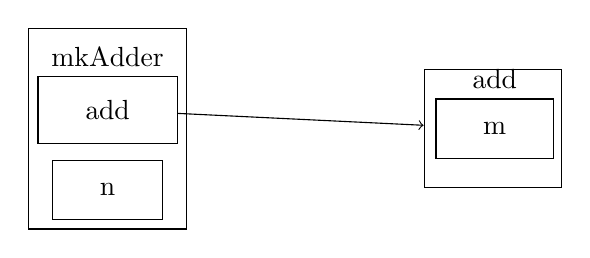
\begin{tikzpicture}[
  mynode/.style = {rectangle, draw, align=center, 
            inner xsep=6mm, inner ysep=3mm}]
  \node [mynode, label={[name=lab1]\lstinline{mkAdder}}] (inner1) {\lstinline{add}};
  \node [mynode, below = 2mm of inner1] (inner2) {\lstinline{n}};
  \node [fit={(inner1) (inner2) (lab1)}, draw] (outer) {};

  \node [mynode, label={[name=lab2]\lstinline{add}}, right = 3.15cm of outer] (inner3) {\lstinline{m}};
  \node [fit={(inner3) (lab2)}, draw, right = 3cm of outer] (outer2) {};

  \path [draw, ->] (inner1) to (outer2);

\end{tikzpicture}

\end{center}

In principle, in a pure functional programming language, none of the pointers in closure structures should be updated. However, as a matter of efficiency,
many functional programming language runtimes use mutation to support certain types of evaluation. Memory tracing, if implemented, could help us understand
``internal mutability'' as a programming language implementation technique.

\subsection{Lazy evaluation and thunks}
Lazy evaluation \citep{LazyEval} is an evaluation strategy and language design technique frequently employed in functional programming languages to support
features such as infinite lists and streams, most notably in the Haskell programming language, which uses lazy evaluation as the default evaluation strategy
\citep{Haskell}.

In Haskell and other lazy programming languages, lazy evaluation is implemented using \emph{thunks}, which are heap-allocated code wrappers\footnote{One could
  also think of thunks as closures without captured environment.}. For each delayed (i.e. non-eager) computation, a thunk is allocated for it. For example, 
\lstinline{cons} (or, in Haskell, \lstinline{(:)}) might wrap each argument in a thunk, forcing the evaluation of either only when requested. This allows
infinite lists to be represented in finite memory.

However, thunk leaks are a major memory problem in Haskell. In Haskell, virtually all calls are lazy, and thus almost every function call wraps its arguments
inside thunks. When a function has a very deep call tree, the number of thunks allocated increases rapidly. Through memory tracing thunks, language implementers
could better understand the ``hot'' locations of trace allocation and deallocation with greater accuracy.

\section{Making sense of functional memory traces}
Although we can add tracing to many functional programming languages by modifying and extending their runtime systems, it is not a trivial task to make sense out
of the traces. Linked data structures and closures usually map to language constructs (i.e., algebraic data types and lexically-scoped functions) quite closely,
but other kinds of heap-allocated structures (such as thunks) might not map to language-level constructs straightforwardly. To make sense of memory traces of
functional programming languages, new labeling mechanisms will need to be devised.


\chapter{Related and Future Work}
\label{chap:conclusion}
\section{Future work}
\subsection{Increasing the accuracy of timestamps}
In \hyperref[subsec:timestamp]{chapter 4}, we gave a formal definition of timestamps. However, intuitive as it might be, this definition actually presumes
one thing that is not true of all programs. Specifically, it presumes that all events are logically sequential and naturally admits a total ordering. This
is, however, not true for many concurrent programs. For example, two events $e_1$ and $e_2$ might be concurrent with each other, and $e_1$ might occur earlier
in one execution profile, while $e_2$ might occur later in another. The timestamp, thus, would depend on execution environment and the scheduler in use.

Instead of imposing total ordering on all events, we may loosen this requirement and instead analyze the set of events as a bounded lattice, where all
suprema correspond to thread joins and all infima correspond to thread forks. Naturally, our timestamps would no longer be natural numbers, but would
instead use more complex mechanisms like Lamport clocks \citep{LamportClock} or vector clocks \citep{VectorClock}. Using vector clocks for dynamic program
analysis is not a new thing \citep{Pacer}, but modifying the Merlin algorithm to use vector clocks is still an open problem. However, without theoretical
advances, the timestamping strategy for concurrent events could not be improved.

\subsection{Porting Elephant Tracks II to other languages}
Elephant Tracks II employs a modular and easily extensible architecture, and in principle any runtime system
that uses heap allocated data structures could be used with Elephant Tracks II. However, for each runtime system, one needs to write a separate frontend
implementation for ET2, which limits the speed at which ET2 could be ported.

Currently, we only have a JVM frontend for ET2, but we have also been considering implementing other frontends. A Haskell frontend is particularly
interesting, in part because Haskell uses lazy evaluation and is notorious for using a lot of heap memory; with Elephant Tracks II, we could better
understand the factors responsible for Haskell's inefficient memory use (or perhaps discover, disappointingly, that there is little space for
improvement). Combined with techniques like dynamic space limits \citep{DynamicSpaceLimits} and strictness inference \citep{Autobahn}, memory tracing could be
used effectively towards optimization of the Glasgow Haskell Compiler's memory usage and leak problems. A Haskell frontend has been a goal of this
project, but unfortunately we have not been able to implement it due to time constraints. Other frontends worth exploring including object-oriented
languages like JavaScript and functional languages like OCaml, but these are currently not our priority.

\section{Related work on object lifetime analysis}
We call Elephant Tracks II a ``memory analysis framework'' because Elephant Tracks II traces could be used
for many different purposes, but at its core, Elephant Tracks II is a lifetime analysis tool. However, there
are many different approaches---which will be briefly discussed here---to lifetime analysis besides the approach that
Elephant Tracks II uses.

\subsection{Static lifetime analysis techniques: regions and region inference}
Elephant Tracks II uses dynamic analysis to determine object lifetimes. As such,
it incurs a heavy runtime penalty such that precise analysis could be conducted, and
that accurate traces could be generated.

Thus, the huge overhead of Elephant Tracks II and other dynamic memory tracing
tools could be prohibitive in real world circumstances. For example, one single
execution of long-running applications like servers and daemons might last days, months
or even years, and it is almost impossible for a programmer to use Elephant Tracks II
to analyze these applications. Naturally, as with any kind of program analysis task, one
might ask if there are \emph{static} instead of \emph{dynamic} approaches to the same task.
In this case, one may be willing to give up some accuracy for efficiency, as analyses could
now be completed at compile time as opposed to at runtime.

The technique for static inference of object lifetimes has long existed. One such algorithm,
\emph{region inference} \citep{RegionInference, StackOfRegions}, is based on the concept of memory ``regions'', which are simply
blocks of heap-allocated memory. In this memory model, heap memory management is based on pushing
and popping a stack of regions: an object is deallocated when its containing region is popped from the
``stack''. In other words, object deallocation times and thus object lifetimes are decided statically. Both
the now-defunct ML Kit Standard ML compiler and the heavily optimizing MLton \citep{MLton} compiler
perform region analysis to complement garbage collection. With some tweaking, one can turn a
region inferencer into an (approximate) ``static memory tracer''.

Although \cite{RegionInference}'s algorithm does support imperative features like reads and writes into references,
the inference rules are still relatively simplistic for more complicated imperative languages. The Cyclone
project attempts to use region inference to determine object lifetime statically in the context of
low-level, imperative programming languages, and has achieved good practical results \citep{Cyclone}. However,
although in many cases the Cyclone compiler could perform region inference automatically, sometimes explicit
region annotations by the programmer are required, making Cyclone incomplete as an object lifetime inference
system.

\subsection{Type-theoretic approach: linear and substructural type systems}
For programming languages theorists and mathematically-inclined programmers, there is an even more straightforward
approach to static object lifetime analysis: that is, to (implicitly) encode lifetime information in objects'
types. One category of such type systems is the \emph{substructural} type systems, which add usage constraints to
its objects: for example, in a \emph{linear} type system, all values must be used exactly once; in an \emph{affine}
type system, a value can be used no more than once \citep{SubstructuralTypes}. If combined with some type
inference, a substructural type system effectively allows for compile-time inference of object lifetimes.

Little has been done in using substructural type systems to determine object lifetimes for real, sensible programs.
However, the Rust programming language \citep{RustLang} has introduced a substructural type system into a systems
programming language, and has been successful in automatically determining lifetimes of values and objects using
type information. However, reference counting is still required in order to achieve reference sharing; moreover, there are
certain cases where the lifetimes of function parameters could not be determined automatically and where manual
annotations are required. Finally, there is no rigorous proof of the correctness of Rust's lifetime analysis, and bugs in the
reference implementation have most certainly been found, but more recently \cite{RustBelt} has proved the correctness and consistency
of a large subset of Rust, which includes many of Rust's lifetime inference rules.

\subsection{Caveats of static analysis methods}
However, one must note that none of the aforementioned static methods could generate perfectly accurate death records for objects,
as a simple corollary of Rice's theorem. For many practical purposes, statically generated ``death records'' are sufficient, but
dynamic analysis is still irreplaceable when preciseness is important (such as when evaluating the performance of garbage collectors).

Moreover, it is extremely difficult to devise static analyses for industry-strength programming languages. It is relatively simple
to devise a region inference algorithm for a well-defined and relatively simple language like Standard ML, but for more complex and
less well-defined functional programming languages such as Haskell, OCaml and Scala --- not to mention imperative programming
languages like Java --- such algorithms will be much harder or even practically impossible to devise. Elephant Tracks II was designed
and developed by a college senior under the advisement of one professor, but even a simple region inference algorithm for a
small subset of Java would be much harder to devise. If one takes into account the human cost of research and development, dynamic
analysis is still, by far, the most effective method to generate memory traces.

\section{The next step: using ET2 for (more) productive purposes}
The main body of this thesis describes the architecture and implementation of Elephant Tracks II, but relatively little is devoted to
explaining why Elepahnt Tracks II is useful. Indeed, as stated in the introduction, memory traces generated by Elephant Tracks II could
and have been used to profile and improve garbage collector performance, detect memory leaks, and instruct programmers about their memory
usage and help them evaluate their programming practices. However, although memory traces could be used for a number of feats, the traces
are of little utility in their raw form: a few gigabytes of cryptic ASCII text. Nevertheless, the great value of memory traces have only been
occasionally explored. This section outlines some potential directions for research and future work in the Elephant Tracks II project and in
memory tracing, in general.

\subsection{Visualization}
The visualization of memory traces is still an open research problem at the moment, although it is difficult to deem the problem ``closed''
any time soon since visualizations could always be improved and new visualizations could always be developed. A simple, intuitive display of
all heap objects over time would be a poor choice, given the large number of allocated objects in a complex enough program; moreover, even if
the number of allocated objects is small, most of the allocated objects are perhaps uninteresting to most programmers. For example, a Scala
programmer is probably not interested in all function closures allocated during program execution.

\cite{Heapviz} presents a tool, Heapviz, that is an improvement to the straightforward approach by providing some summarization facilities,
allowing programmers to view a simplified and much more useful version of the heap graph. However, Heapviz is still not good enough: for example,
it does not describe memory properties quantitatively, and it provides little helps for programmers to \emph{improve} their programs based on
the traces that they have collected. To fully harvest the information hidden in memory traces and make them available to programmers, we need a
more powerful visualization tool, which does not exist as of yet. However, a team including this author has been working on a new visualizer for
Elephant Tracks and Elephant Tracks II, which should provide more functionality than Heapviz.

\subsection{Memory traces as a programming language}
Memory traces could be though as code for a very simple programming language operating on heap objects akin to C structures, with three basic operations:
object allocation, pointer update, and object death (``deallocation''). The GC simulator in Elephant Tracks II could thus be thought of as an
interpreter for this programming language. Although the GC trace language is not a practical or useful language for programming, this small insight
allows us to use memory traces the way one uses a program.

\subsection{Abstraction and analysis}
There are many useful techniques to reason about and analyze the behavior of pointers and heap objects. Some more prominent ones include separation
logic \citep{SeparationLogic}, shape analysis \citep{ShapeAnalysis}, and escape analysis. However, writing such analyses for full programs could be
tedious. Given that a memory trace is a simplified version of a full imperative program that preserves only its heap properties, we might be able to
run static analyses on and verify program properties with those traces instead. For example, instead of running shape analysis on a Java program, one
might want to instead run shape analysis on its trace to detect certain classes of memory bugs. However, little work has been done in this field at the
time of the publication of this thesis.

\subsection{Extracting useful information from memory traces}
Memory traces contain a lot of useful information, but relatively little of that has been utilized. \cite{MemInsight} used memory traces to detect the
presence of memory leaks in JavaScript programs, but much more information could be extracted from memory traces. Some of these information can be easy
to extract: with a little bit of effort, one could determine the ``cost centers'' of a program given a trace, or methods/functions where most memory is
allocated; one can also obtain a time-function of heap size easily.

However, more interesting and useful information can be much harder to harvest. Since Elephant Tracks II records the thread associated with each trace
entry, one could potentially use Elephant Tracks to discover race conditions in programs. Moreover, as ET2 traces provides accurate object death
records, those traces could be used as heuristic hints for the garbage collector. Using techniques akin to shape analysis, one could discover the
data structures used in the program. None of these potential uses of memory traces have been explored as of yet (due to the cost-ineffectiveness of not
having a good memory tracer), but Elephant Tracks II should enable some more productive uses of memory traces.

\subsection{Combining static and dynamic analysis}
Memory tracing is a form of dynamic analysis, but it can also be enhanced by static analyses. For example, if combined with escape analysis and liveness
analysis, we can potentially make tracing more efficient, while also producing more accurate traces. No work, however, has been done in this
field as of now.


\chapter{Conclusion}
\label{chap:realconclusion}
\section{Related work on object lifetime analysis}
We call Elephant Tracks II a ``memory analysis framework'' because Elephant Tracks II traces could be used
for many different purposes, but at its core, Elephant Tracks II is a lifetime analysis tool. However, there
are many different approaches---which will be briefly discussed here---to lifetime analysis besides the approach that
Elephant Tracks II uses.

\subsection{Static lifetime analysis techniques: regions and region inference}
Elephant Tracks II uses dynamic analysis to determine object lifetimes. As such,
it incurs a heavy runtime penalty such that precise analysis could be conducted, and
that accurate traces could be generated.

Thus, the huge overhead of Elephant Tracks II and other dynamic memory tracing
tools could be prohibitive in real world circumstances. For example, one single
execution of long-running applications like servers and daemons might last days, months
or even years, and it is almost impossible for a programmer to use Elephant Tracks II
to analyze these applications. Naturally, as with any kind of program analysis task, one
might ask if there are \emph{static} instead of \emph{dynamic} approaches to the same task.
In this case, one may be willing to give up some accuracy for efficiency, as analyses could
now be completed at compile time as opposed to at runtime.

The technique for static inference of object lifetimes has long existed. One such algorithm,
\emph{region inference} \citep{RegionInference, StackOfRegions}, is based on the concept of memory ``regions'', which are simply
blocks of heap-allocated memory. In this memory model, heap memory management is based on pushing
and popping a stack of regions: an object is deallocated when its containing region is popped from the
``stack''. In other words, object deallocation times and thus object lifetimes are decided statically. Both
the now-defunct ML Kit Standard ML compiler and the heavily optimizing MLton \citep{MLton} compiler
perform region analysis to complement standard garbage collection. With some tweaking, one can turn a
region inferencer into an (approximate) ``static memory tracer''.

Although \cite{RegionInference}'s algorithm does support imperative features like reads and writes into references,
the inference rules are still relatively simplistic for more complicated imperative languages. The Cyclone
project attempts to use region inference to determine object lifetime statically in the context of
low-level, imperative programming languages, and has achieved good practical results \citep{Cyclone}. However,
although in many cases the Cyclone compiler could perform region inference automatically, sometimes explicit
region annotations by the programmer are required, making Cyclone incomplete as an object lifetime inference
system.

\subsection{Type-theoretic approach: linear and substructural type systems}
For programming languages theorists and mathematically-inclined programmers, there is an even more straightforward
approach to static object lifetime analysis: that is, to (implicitly) encode lifetime information in objects'
types. One category of such type systems is the \emph{substructural} type systems, which add usage constraints to
its objects: for example, in a \emph{linear} type system, all values must be used exactly once; in an \emph{affine}
type system, a value can be used no more than once \citep{SubstructuralTypes}. If combined with some type
inference, a substructural type system effectively allows for compile-time inference of object lifetimes.

Little has been done in using substructural type systems to determine object lifetimes for real, sensible programs.
However, the Rust programming language \citep{RustLang} has introduced aspects of substructural types into a systems
programming language, and has been successful in automatically determining lifetimes of values and objects using
type information. However, reference counting is still required in order to achieve reference sharing; moreover, there are
certain cases where the lifetimes of function parameters could not be determined automatically and where manual
annotations are required. Finally, there is no rigorous proof of the correctness of Rust's lifetime analysis, and bugs in the
reference implementation have most certainly been found, but more recently \cite{RustBelt} has proved the correctness and consistency
of a large subset of Rust, which includes many of Rust's lifetime inference rules.

\subsection{Caveats of static analysis methods}
However, one must note that none of the aforementioned static methods could generate perfectly accurate death records for objects,
as a simple corollary of Rice's theorem. For many practical purposes, statically generated ``death records'' are sufficient, but
dynamic analysis is still irreplaceable when preciseness is important (such as when evaluating the performance of garbage collectors).

Moreover, it is extremely difficult to devise static analyses for industry-strength programming languages. It is relatively simple
to devise a region inference algorithm for a well-defined and relatively simple language like Standard ML, but for more complex and
less well-defined functional programming languages such as Haskell, OCaml and Scala --- not to mention imperative programming
languages like Java --- such algorithms will be much harder or even practically impossible to devise. Elephant Tracks II was designed
and developed by a college senior under the advisement of one professor, but even a simple region inference algorithm for a
small subset of Java would be much harder to devise. If one takes into account the human cost of research and development, dynamic
analysis is still, by far, the most effective method to generate memory traces.

\section{The next step: using ET2 for (more) productive purposes}
The main body of this thesis describes the architecture and implementation of Elephant Tracks II, but relatively little is devoted to
explaining why Elepahnt Tracks II is useful. Indeed, as stated in the introduction, memory traces generated by Elephant Tracks II could
and have been used to profile and improve garbage collector performance, detect memory leaks, and instruct programmers about their memory
usage and help them evaluate their programming practices. However, although memory traces could be used for a number of feats, the traces
are of little utility in their raw form: a few gigabytes of cryptic ASCII text. Nevertheless, the great value of memory traces have only been
occasionally explored. This section outlines some potential directions for research and future work in the Elephant Tracks II project and in
memory tracing, in general.

\subsection{Visualization}
The visualization of memory traces is still an open research problem at the moment, although it is difficult to deem the problem ``closed''
any time soon since visualizations could always be improved and new visualizations could always be developed. A simple, intuitive display of
all heap objects over time would be a poor choice, given the large number of allocated objects in a complex enough program; moreover, even if
the number of allocated objects is small, most of the allocated objects are perhaps uninteresting to most programmers. For example, a Scala
programmer is probably not interested in all function closures allocated during program execution.

\cite{Heapviz} presents a tool, Heapviz, that is an improvement to the straightforward approach by providing some summarization facilities,
allowing programmers to view a simplified and much more useful version of the heap graph. However, Heapviz is still not good enough: for example,
it does not describe memory properties quantitatively, and it provides little helps for programmers to \emph{improve} their programs based on
the traces that they have collected. To fully harvest the information hidden in memory traces and make them available to programmers, we need a
more powerful visualization tool, which does not exist as of yet. However, a team including this author has been working on a new visualizer for
Elephant Tracks and Elephant Tracks II, which should provide more functionality than Heapviz.

\subsection{Memory traces as a programming language}
Memory traces could be though as code for a very simple programming language of heap objects akin to C structures, with three basic operations:
object allocation, pointer update, and object death (``deallocation''). The GC simulator in Elephant Tracks II could thus be thought of as an
interpreter for this programming language. Although the GC trace language is not a practical or useful language for programming, this small insight
allows us to use memory traces the way one uses a program.

\subsection{Abstraction and analysis}
There are many useful techniques to reason about and analyze the behavior of pointers and heap objects. Some more prominent ones include separation
logic \citep{SeparationLogic}, shape analysis \citep{ShapeAnalysis}, and escape analysis. However, writing such analyses for full programs could be
tedious. Given that a memory trace is a simplified version of a full imperative program that preserves only its heap properties, we might be able to
run static analyses on and verify program properties with those traces instead. For example, instead of running shape analysis on a Java program, one
might want to instead run shape analysis on its trace to detect certain classes of memory bugs. However, little work has been done in this field at the
time of the publication of this thesis.

\subsection{Extracting useful information from memory traces}
Memory traces contain a lot of useful information, but relatively little of that has been utilized. \cite{MemInsight} used memory traces to detect the
presence of memory leaks in JavaScript programs, but much more information could be extracted from memory traces. Some of these information can be easy
to extract: with a little bit of effort, one could determine the ``cost centers'' of a program given a trace, or methods/functions where most memory is
allocated; one can also obtain a time-function of heap size easily.

However, more interesting and useful information can be much harder to harvest. Since Elephant Tracks II records the thread associated with each trace
entry, one could potentially use Elephant Tracks to discover race conditions in programs. Moreover, as ET2 traces provides accurate object death
records, those traces could be used as heuristic hints for the garbage collector. Using techniques akin to shape analysis, one could discover the
data structures used in the program. None of these potential uses of memory traces have been explored as of yet (due to the cost-ineffectiveness of not
having a good memory tracer), but Elephant Tracks II should enable some more productive uses of memory traces.

\subsection{Combining static and dynamic analysis}
Memory tracing is a form of dynamic analysis, but it can also be enhanced by static analyses. For example, if combined with escape analysis and liveness
analysis, we can potentially make tracing more efficient, while also producing more accurate traces. No work, however, has been done in this
field as of now.

\subsection{Porting Elephant Tracks II to other languages}
Finally, it is worth mentioning that Elephant Tracks II employs a modular and easily extensible architecture, and in principle any runtime system
that uses heap allocated data structures could be used with Elephant Tracks II. However, for each runtime system, one needs to write a separate frontend
implementation for ET2, which limits the speed at which ET2 could be ported.

Currently, we only have a JVM frontend for ET2, but we have also been considering implementing other frontends. A Haskell frontend is particularly
interesting, in part because Haskell uses lazy evaluation and is notorious for using a lot of heap memory; with Elephant Tracks II, we could better
understand the factors responsible for Haskell's inefficient memory use (or perhaps discover, disappointingly, that there is little space for
improvement). Combined with techniques like dynamic space limits \citep{DynamicSpaceLimits} and strictness inference \citep{Autobahn}, memory tracing could be
used effectively towards optimization of the Glasgow Haskell Compiler's memory usage and leak problems. A Haskell frontend has been a goal of this
project, but unfortunately we have not been able to implement it due to time constraints. Other frontends worth exploring including object-oriented
languages like JavaScript and functional languages like OCaml, but these are currently not our priority.

\section{Conclusion}
Memory tracing is a useful and valuable dynamic analysis that can help programmers understand how they use heap memory in their programs, but it has
also been a very costly and particularly inefficient analysis to perform, making it impractical for most purposes. In light of this problem, this thesis
presents a tool, Elephant Tracks II, that is designed to make memory tracing useful again. To attain this goal, Elephant Tracks II uses an extensible, modular
design, and the JVM frontend for Elephant Tracks II particularly benefits from the modular architecture to improve the performance of memory tracing. In short,
the Elephant Tracks II project and this thesis's contributions are as following:
\begin{itemize}
\item providing an efficient memory tracing tool for Java;
\item developing an modular and effective architecture for memory tracing;
\item enhanced the understanding of memory behavior of functional programs;
\item demonstrated the need for careful planning and design in research software;
\item highlighted the importance of good engineering practices in research programming.
\end{itemize}

In the final analysis, the Elephant Tracks II project makes several important contributions not only to the field of dynamic analysis, but also to the
practice of research programming in general. Elephant Tracks II does not only provide an important and effective tool for memory tracing, but also
illustrates good practice and its importance in research programming. However, a little goes a long way: Elephant Tracks II makes it possible for program
analysis researchers and practitioners to analyze memory usage more easily, but we are still on our way to fully discover the value of memory tracing and of
Elephant Tracks II as a tool.


\chapter*{Appendix: Overview of Code Repositories}
\addcontentsline{toc}{chapter}{Appendix: Overview of Code Repositories}
\label{appendix:a}
All code written for this thesis is open-sourced and publicly available on GitHub.

\section{The red-black tree benchmark}
The red-black tree benchmark is a simple benchmark used to investigate and benchmark behavior in functional programming
systems and runtime systems. The benchmark has been ported to four languages: Scala, Haskell, Standard ML, and OCaml. We
used the four ports to benchmark four runtime systems: the HotSpot JVM \& Oracle JDK, the Glasgow Haskell Compiler (GHC),
MLton, and the INRIA reference OCaml implementation, respectively.

The red-black tree benchmark consists of three tasks: inserting one million numbers (the integers 1 to 1,000,000) into
an empty red-black tree, printing the height of the red-black tree, and then in-order traversing the red-black tree. The
implementation of the red-black tree is based on \cite{PFDS}'s purely functional implementation.

For code and build instructions, please visit: ~\url{https://github.com/ElephantTracksProject/rbtbench}.

\section{The Java micro-benchmark suite}
The Java micro-benchmark suite is intended to benchmark the Java frontend to Elephant Tracks 2. It consists of the
following benchmarks, the first five of which are written in Java and the latter two written in Scala:
\begin{itemize}
\item \lstinline{Hello}: the ``Hello, world!'' program;
\item \lstinline{BF}: implements an interpreter for an esoteric, minimal programming language;
\item \lstinline{BinarySearchTree}: builds two standard, imperative binary search trees, inserts two sets of data into them,
in-order traverses them, and calculate their respective heights;
\item \lstinline{LambdaCalc}: implements a simple untyped, call-by-value $\lambda$-calculus evaluator using a simple named representation, and attempts
to $\beta$-reduce the $\lambda$-term $(\lambda x \ . \ (x \ x)) \ (\lambda y \ . \ y) \ (\lambda z \ . \ z)$.
\item \lstinline{NatArith}: implements inductive natural number arithmetic (i.e., as implemented in Coq and Idris) and
conversion between natural numbers and Java integers, and evaluates $1921 + 3385$ using the implementation;
\item \lstinline{FunctionalCounter}: implements a counter using closure capture of local variables, and invokes the counter
a large number of times;
\item \lstinline{FunctionalRBT}: the same Scala red-black tree benchmark from the red-black tree benchmark suite.
\end{itemize}

For code and build instructions, please visit: ~\url{https://github.com/ElephantTracksProject/benchmarks}.

\section{Elephant Tracks II}
ET2 is contained in multiple repositories. The Java frontend is located at: ~\url{https://github.com/ElephantTracksProject/et2-java}.
Our fork of the JNIF library, which is needed to build the Java frontend, is located at: ~\url{https://github.com/ElephantTracksProject/jnif}.


\bibliographystyle{acmref}
\bibliography{thesis}
\end{document}
